
%% Template by Michal Forisek


\documentclass[12pt,a4paper]{book}
\usepackage{slovak}
\usepackage[utf8]{inputenc}
\usepackage{a4wide}
\usepackage{tabularx}
\usepackage{amsfonts}
\usepackage{amssymb}
\usepackage{amsmath}
\usepackage{epsfig}
\usepackage{color}
\usepackage{mathrsfs}
\usepackage{verbatim}
\usepackage{hyperref}
\usepackage{subfigure}
\usepackage{float}
\usepackage{longtable}
\usepackage{listings}
\usepackage{graphicx}
\usepackage{mathtools}
% vim: set fdm=marker:
%% Original by Michal Forisek

%% zakladne definicie
\newcommand{\quoteme}[1]{\clqq#1\crqq}
\def\todo#1{[{\color{red} TODO:} {\bf  #1}]}
\def\fixme#1{[{\color{red} FIXME:} {\bf  #1}]}
\def\verify#1{\todo{verify: #1}}
\DeclarePairedDelimiter{\ceil}{\lceil}{\rceil}
\DeclarePairedDelimiter{\floor}{\lfloor}{\rfloor}


\def\xor{\oplus}
\def\concat{\|}
%\def\inr{\in_{R}}
\def\toa #1 {\overset{#1}{\rightarrow}}
\def\inr{\overset{\$}{\leftarrow}}
\def\assign{\leftarrow}
\def\send{\rightarrow}
\def\isomorph{\cong}
\def\nsd{NSD}
\def\union{\cup}
\newcommand{\unit}[1]{\ensuremath{\, \mathrm{#1}}}
\DeclareMathOperator{\dlog}{dlog}

\def\compactlist{
  \setlength{\itemsep}{1pt}
  \setlength{\parskip}{0pt}
  \setlength{\parsep}{0pt}
}
\def\mod{\,{\rm mod}\,}

%%% original od Misofa:
%% {{{

\catcode`\@=11

\def\R{{\cal R}}
\def\cent{{c\kern-0.3em|\kern0.1em}}
\def\N{{N}} % FIXME FIXME 

\let\eps=\varepsilon

\def\relupdown#1#2#3{\mathrel{\mathop{#1}\limits^{#2}_{#3}} }

\let\then=\Rightarrow
\let\neht=\Leftarrow

\def\krok#1{\relupdown{\Longrightarrow}{}{#1}}
\def\thenrm{\relupdown{\Longrightarrow}{}{rm}}

\def\bicik{\upharpoonright}
\def\B{{\mathbf B}}
\def\kodTS#1{{\tt <}#1{\tt >}}

\newtheorem{definicia}{Definícia}[section]
\newtheorem{HLPpoznamka}{Poznámka}[section]
\newtheorem{HLPpriklad}{Príklad}[section]
\newtheorem{HLPcvicenie}[HLPpriklad]{Cvičenie}
\newtheorem{zadanie}{Úloha}[section]
\newenvironment{poznamka}{\begin{HLPpoznamka}\rm}{\end{HLPpoznamka}}
\newenvironment{priklad}{\begin{HLPpriklad}\rm}{\end{HLPpriklad}}
\newenvironment{cvicenie}{\begin{HLPcvicenie}\rm}{\end{HLPcvicenie}}
\newtheorem{veta}{Veta}[section]
\newtheorem{lema}[veta]{Lema}
\newtheorem{dosledok}[veta]{Dôsledok}
\newtheorem{teza}[veta]{Téza}
% \newtheorem{dokaz}{Dôkaz}[section]

\long\def\odsadene#1{
\leftskip=\parindent
\parindent=0pt
\vskip-5pt

\parskip=5pt
#1
\parskip=0pt

\parindent=\leftskip
\leftskip=0pt

} % end \odsadene




%%%%%%%%%%% PROSTREDIE PRE PISANIE KOMENTAROV

%\newenvironment{komentar}{%
%\vskip\baselineskip
%\tabularx{0.95\textwidth}{|X|}
%\sl
%}
%{\endtabularx
%\vskip\baselineskip
%}

\newenvironment{komentar}{%
\vskip\baselineskip\noindent
\tabularx{\textwidth}{>{\hsize=.2\hsize}X>{\hsize=1.8\hsize}X}
\sl ~ & \sl
}
{\endtabularx
\vskip\baselineskip
}

%\newenvironment{komentar}{%
%\vskip\baselineskip
%\trivlist\vspace{-4pt}\raggedleft\item\relax\tabularx{0.9\textwidth}{X}\sl}
%{\endtabularx\vspace{-4pt}\endtrivlist
%\vskip\baselineskip
%}

\newenvironment{dokaz}{\trivlist
  \item[\hskip \labelsep{\bfseries Dôkaz.}]}{\endtrivlist}
  
%\newenvironment{dokaz}{%
%\vskip\baselineskip\noindent
%\tabularx{\textwidth}{||X||}
%\sl
%}
%{\endtabularx
%\vskip\baselineskip
%}

%%%%%%%%%%% PROSTREDIE PRE MOJE ITEMIZE 

\newenvironment{myitemize}{%
\begin{itemize}
\itemsep-3pt
}
{\end{itemize}
}

%%%%%%%%%%% MATICKE MAKRA

\font\tenrm=csr10

\def\eps{\varepsilon}
% \def\R{{\mathbb R}}
\def\lvec#1{\overrightarrow{#1}}
\def\uhol{{\measuredangle}}
\def\then{\Rightarrow}
% \def\lg{{\rm lg}}
\def\lg{\log_2}
%\def\div{\mathbin{\rm div}}
\def\div{{\rm div}}

%%%%%%%%%%% PDF

\newif\ifpdf
\ifx\pdfoutput\undefined
  \pdffalse
\else
  \pdfoutput=1 \pdftrue
\fi

%%%%%%%%%%% OBRAZKY 

\newcommand{\myincludegraphics}[2][]{\includegraphics[#1]{images/#2}}

%%%%%%%%%%% SLOVNICEK

\openout2=\jobname.slo

\newcommand{\definuj}[3][]{%
\def\tmpvoid{}\def\tmpfirst{#1}%
\ifx\tmpvoid\tmpfirst%
  {\sl #2}\label{definicia:#2}\write2{#2 & #3 & \pageref{definicia:#2} \cr}%
\else%
  {\sl #2}\label{definicia:#2}\write2{#1 & #3 & \pageref{definicia:#2} \cr}%
\fi}

\newcommand{\definujsilent}[2]{%
\label{definicia:#1}\write2{#1 & #2 & \pageref{definicia:#1} \cr}%
}

\newcommand\myglossary{
  \immediate\closeout2 
  %\if@twocolumn\@restonecoltrue\onecolumn\else\@restonecolfalse\fi
  \chapter{Slovníček pojmov}
  \begin{tabular}{|l|l|r|}
  \hline
  {\bfseries slovenský pojem} & {\bfseries anglický preklad} & {\bfseries str.} \\ 
  \hline
  \InputIfFileExists{\jobname.srs}{}{~ & ~ & ~ \\}
  \hline
  \end{tabular}
  %\if@restonecol\twocolumn\fi
}

%%%%%%%%%%% UVODZOVKY

\catcode`\"=13
\def "{\begingroup\clqq\def "{\endgroup\crqq}}
\def\dospecials{\do\ \do\\\do\{\do\}\do\$\do\&%
  \do\#\do\^\do\^^K\do\_\do\^^A\do\%\do\~\do\"}

%%%%%%%%%%% DANGER BENDS 

\font\manual=manfnt % font used for the METAFONT logo, etc.
\def\dbend{{\manual\char127}} % dangerous bend sign

\newlength{\bendwidth}   \settowidth{\bendwidth}{\dbend}    \newlength{\hangwidth}

\def\hangone{%
  \hangwidth=\bendwidth%
  \advance\hangwidth 5pt%
  \hangindent\hangwidth%
}
\def\hangtwo{%
  \hangwidth=\bendwidth%
  \multiply\hangwidth 2%
  \advance\hangwidth 6pt% 
  \hangindent\hangwidth%
}

\def\medbreak{\par\ifdim\lastskip<\medskipamount \removelastskip\penalty-100\medskip\fi}
\let\endgraf=\par

\def\d@nger{\medbreak\begingroup\clubpenalty=10000
%\def\d@nger{\begingroup\clubpenalty=10000
%  \def\par{\endgraf\endgroup\medbreak} \noindent\hangone\hangafter=-2
  \def\par{\endgraf\endgroup} \noindent\hangone\hangafter=-2
  \hbox to0pt{\hskip-\hangindent\dbend\hfill}}
\outer\def\danger{\d@nger}

\def\dd@nger{\medbreak\begingroup\clubpenalty=10000
%  \def\par{\endgraf\endgroup\medbreak} \noindent\hangtwo\hangafter=-2
  \def\par{\endgraf\endgroup} \noindent\hangtwo\hangafter=-2
  \hbox to0pt{\hskip-\hangindent\dbend\kern1pt\dbend\hfill}}
\outer\def\ddanger{\dd@nger}

\def\enddanger{\endgraf\endgroup} % omits the \medbreak
\def\enddangerhop{\endgraf\endgroup\medbreak}




\def\@nakedcite#1#2{{#1\if@tempswa , #2\fi}}
\DeclareRobustCommand\nakedcite{%
  \@ifnextchar [{\@tempswatrue\@nakedcitex}{\@tempswafalse\@nakedcitex[]}}
\def\@nakedcitex[#1]#2{%
  \let\@citea\@empty
  \@nakedcite{\@for\@citeb:=#2\do
    {\@citea\def\@citea{,\penalty\@m\ }%
     \edef\@citeb{\expandafter\@firstofone\@citeb\@empty}%
     \if@filesw\immediate\write\@auxout{\string\citation{\@citeb}}\fi
     \@ifundefined{b@\@citeb}{\mbox{\reset@font\bfseries ?}%
       \G@refundefinedtrue
       \@latex@warning
         {Citation `\@citeb' on page \thepage \space undefined}}%
       {\hbox{\csname b@\@citeb\endcsname}} }}{#1}}

\long\def\FIXME#1{
  \begin{center}
  \begin{minipage}{0.8\textwidth}
  {\bf FIXME:~}\sl #1
  \end{minipage}
  \end{center}
}


\catcode`\@=12
%% }}}


\linespread{1.2}

\begin{document}

% Obal
\thispagestyle{empty}
\begin{minipage}{0.25\textwidth}

\includegraphics[width=0.9\textwidth]{img/komlogo-new}
\end{minipage}
\begin{minipage}{0.69\textwidth}
\begin{center}
UNIVERZITA KOMENSKÉHO V BRATISLAVE \\
FAKULTA MATEMATIKY, FYZIKY A INFORMATIKY \\
\end{center}
\end{minipage}

\bigskip
TODO mozno kod

\vfill
\begin{center}
\begin{minipage}{0.8\textwidth}
%\hrule
\bigskip\medskip
\centerline{\LARGE\sc Problém dvoch obchodných cestujúcich}
\end{minipage}
\end{center}
\vfill
{\bf 2013}

\hfill{\bf Vladimír Boža}
\eject % EOP i

%Titulna strana
\thispagestyle{empty}
\begin{minipage}{0.25\textwidth}

\includegraphics[width=0.9\textwidth]{img/komlogo-new}
\end{minipage}
\begin{minipage}{0.69\textwidth}
\begin{center}
UNIVERZITA KOMENSKÉHO V BRATISLAVE \\
FAKULTA MATEMATIKY, FYZIKY A INFORMATIKY \\
\end{center}
\end{minipage}

\vfill
\begin{center}
\begin{minipage}{0.8\textwidth}
%\hrule
\bigskip\medskip
\centerline{\LARGE\sc Problém dvoch obchodných cestujúcich}
\smallskip
\centerline{(diplomová práca)}
\bigskip
\bigskip
%\centerline{\large\sc Vladimír Boža}
\bigskip\bigskip
%\hrule
\end{minipage}
\end{center}
\vfill
\begin{tabular}{l l}
Študijný program: & Informatika \\
Študijný odbor: & 9.2.1 Informatika \\
Školiace pracovisko: & Katedra informatiky \\
Školiteľ: & RNDr. Michal Forišek PhD. \\
\end{tabular}
\vfill
{\bf Bratislava, 2013}

\hfill{\bf Vladimír Boža}
\eject % EOP i

%\thispagestyle{empty}
%\includegraphics[scale=0.7]{zad.pdf}
%\eject

\thispagestyle{empty}

\section*{Abstrakt}

TODO

\medskip
{\bf Kľúčové slová:} TODO
\eject

\thispagestyle{empty}

\section*{Abstract}

TODO engrish

\medskip
{\bf Key words:} TODO
\eject

\thispagestyle{empty}
\tableofcontents
\thispagestyle{empty}

\setcounter{page}{0}
\chapter*{Úvod}
\addcontentsline{toc}{chapter}{Úvod}
\label{chapter:uvod}
TODO


\chapter{Definícia problému}
\label{chapter:definition}
V tejto kapitole formálne zadefinujeme problém dvoch obchodných cestujúcich
a jeho variácie, ktoré budeme riešiť.

\begin{definicia}[Problém dvoch obchodných cestujúcich]
Majme daný úplný ohodnotený graf $G = (V, E)$ s $n$ vrcholmi, pričom každá hrana
$e \in E$ má dĺžku $c(e)$. Cieľom je nájsť dve hranovo disjuktné hamiltonovské kružnice
$K_1 \subset E$, $K_2 \subset E$, tak aby súčet ich dĺžok bol minimálny.
Kružnice $K_1, K_2$ budeme volať aj TSP-cesty.
\end{definicia}

\begin{poznamka}
Cenu hranu spájajúcej vrcholy $u, v$ budeme označovať ako $c(u, v)$. 
\end{poznamka}

V niektorých prípadoch kladieme na dĺžky hrán ďalšie obmedzenia.
Jedným z obmedzení je trojuholníková nerovnosť:

\begin{definicia}{Trouholníková nerovnosť}
Hrany uhodnoteného grafu $G = (V, E)$ splňajú trouholníkovú nerovnosť, ak platí:
$$\forall u,v,w \in V: c(u,v) + c(v,w) \geq c(u,w)$$
\end{definicia}

Ešte silnejším obmedzením je požadovať, aby vrcholy grafu zodpovedali bodom v rovine, t.j.
každému vrcholu priradíme reálne čísla $x_v, y_v$ a vzdialenosť vrcholov $u, v$ bude:
$\sqrt{(x_u - x_v)^2 + (y_u - y_v)^2}$.


\chapter{Doterajšie výsledky}
\label{chapter:previous}
Problém dvoch obchodných cestujúcich je zjavne NP-úplný, ako to dokázal
už \cite{krarup}, keď tento problém zadefinoval.

V nasledujúcich riadkoch uvedieme niekoľko doterajších výsledkoch, ktoré sa vyskytli
pri riešení tohoto problému.

\section{Aproximačné algoritmy}

Dá sa pomerne ľahko ukázať, že pre problém dvoch obchodných cestujúcich vo všeobecných grafoch
neexistuje aproximačný algoritmus s konštantným aproximačným pomerom. Dôkaz je v prakticky
rovnaký ako pre problém obchodného cestujúceho.

V prípade, že graf spĺňa trojuholníkovu nerovnosť sa už dajú nájsť approximačné algoritmy.
Dá sa napríklad ukázať, že ak má graf dostatočne veľa vrcholov, tak ku každej TSP ceste
existuje TSP cesta, ktorá je s ňou disjuktná a má dĺžku najviac rovnú $(2+\epsilon)$-násobku
dĺžky pôvodnej cesty.
Použítím $1.5$-aproximácie pre problém obchodného cestujúceho (\cite{christofides}) vieme
dostať $(9/4 + \epsilon)$-aproximačný algoritmus. 

Dá dosiahnúť aj $2$-aproximačný algoritmus, ako to je ukázané v \cite{apx2}. Hlavnou
ideou je zostrojiť najprv dve disjuktné kostry s minimálnou cenou pomocou algoritmu
uvedeného v \cite{spanning2} a následne pomerne technickou konštrukciou zostrojiť
s použitím týchto kostier dve disjunktné hamiltonovské kružnice.

V prípade, že ceny hrán môžu byť len z množiny $\{1,2\}$ existuje $11/9$-aproximačný
algoritmus (\cite{gimadi}). V tomto článku sa nachádza navyše niekoľko výsledkov pre 
variáciu problému, kde cenu ciest maximalizujeme.

\section{Riešenia pomocou celočíselného lineárneho programovania}

\subsection{Riešenie problému obchodného cestujúceho pomocou celočíselného
lineárneho programovania}

Najprv zhrnieme niekoľko výsledkov o riešení problému obchodného cestujúceho pomocou
celočíselného lineárneho programovania, ktoré sa nachádzajú v \cite{tspsurvey}.

Problém obchodného cestujúceho sa dá priamočiaro popísať nasledujúcim celočíselným lineárnym
programom:

$$\min \sum_{e \in E} c(e) x_e$$ 

Za predpokladov:
\begin{subequations}
\begin{equation}\forall e \in E: x_e \in \{0, 1\} \label{eq:enum}\end{equation}
\begin{equation}\forall v \in V: \sum_{e \in \delta(v)} x_e = 2 \label{eq:vertexsum1} \end{equation}
\begin{equation}\forall S \subset V, S \neq \emptyset: \sum_{e \in \delta(S)} x_e \geq 2 \label{eq:subtour1}\end{equation}
\end{subequations}

Kde $\delta(v)$ je množina všetkých hrán, ktoré majú koniec vo vrchole $v$ a
$\delta(S)$ je množina všetkých hrán, ktorá majú jeden koniec v $S$ a druhý v $V \setminus S$.

Podmienky \eqref{eq:vertexsum1} zabezpečujú, aby z každého vrchola výchádzali práve
dve hrany. Podmienky \eqref{eq:subtour1} zabezpečujú, aby sme mali iba jeden cyklus.
Táto formulácia má ale exponenciálne veľa podmienok a na prvý pohľad je neužitočná.

Existuje formulácia, ktorá má iba polynomiálne veľa podmienok. V tomto prípade
ale použijeme orientované hrany:

$$\min \sum_{i\neq j} c(i,j) x_{ij}$$

Za predpokladov:
\begin{subequations}
\begin{equation}\forall j \neq i_0: \sum_{i=1}^n x_{ij} = 1\end{equation}
\begin{equation}\forall i \neq i_0: \sum_{j=1}^n x_{ij} = 1\end{equation}
\begin{equation}\forall i,j, i \neq i_0 \vee j \neq j_0: u_i + u_j + nx_{ij} \leq n-1\end{equation}
\end{subequations}

Cieľom premenných $u_i$ je zaviesť očíslovanie vrcholov na kružnici. Tento program
má síce len polynomiálne veľa podmienok, ale ukazuje sa, že nie je ľahko riešiteľné
pomocou bežných nástrojov na riešenie celočíselných lineárnych programov.

Ukazuje sa, že pomerne účinný algoritmus je nasledovný:

\begin{enumerate}
\item Vytvor lineárny program, ktorá obsahuje iba podmienky \eqref{eg:enum}, 
\eqref{eq:vertexsum1}.
\item Najdi riešenie daného lineárneho programu.
\item Ak je riešenie lineárneho programu iba jedna kružnica, tak máme dobré riešenie a skonči.
\item Ináč nájdi porušené podmienky \eqref{eq:subtour1} a pridaj ich do lineárneho
programu. A pokračuj krokom 2.
\end{enumerate}

Tomuto postupu sa zvykne hovoriť aj "subtour elimination".

\subsection{Riešenie problému dvoch obchodných cestujúcich pomocou celočíselného
lineárneho programovania}

V nasledujúcej časti zhrnieme výsledky z \cite{duchenne}.
Priamym rozšírením postupu pre obchodného cestujúceho na dvoch cestujúcich
dostaneme nasledovný program:

$$\min \sum_{e \in E} c(e) x_e + \sum_{e \in E} c(e) y_e$$ 

Za predpokladov:
\begin{subequations}
\begin{equation}\forall e \in E: x_e \in \{0, 1\}\end{equation}
\begin{equation}\forall e \in E: y_e \in \{0, 1\}\end{equation}
\begin{equation}\forall e \in E: x_e + y_e \leq 1\end{equation}
\begin{equation}\forall v \in V: \sum_{e \in \delta(v)} x_e = 2\end{equation}
\begin{equation}\forall v \in V: \sum_{e \in \delta(v)} y_e = 2\end{equation}
\begin{equation}\forall S \subset V, S \neq \emptyset: \sum_{e \in \delta(S)} x_e \geq 2
\label{eq:subtour2}\end{equation}
\begin{equation}\forall S \subset V, S \neq \emptyset: \sum_{e \in \delta(S)} y_e \geq 2
\label{eq:subtour3}\end{equation}
\end{subequations}

Spôsob riešenie je podobný ako pri riešení problému obchodného cestujúceho -- najprv
nepoužijeme žiadne z podmienok \eqref{eq:subtour2}, \eqref{eq:subtour3} a postupne
pridáme len porušené podmienky. V \cite{duchenne} sa tento algoritmus nazýva "3-index".

Ukazuje sa, že tento algoritmus je pomerne pomalý a potrebuje veľa iterácií riešenia
lineárneho programu. Pri praktickom testovaní na náhodných euklidovských grafoch
je tento algoritmus úspešný maximálne pre grafy s $50$ vrcholmi. Hlavným problémom
tohoto algoritmu je, že pomerne často nastáva taký prípad, keď len prehadzujeme hrany z $x$ 
do $y$ a naopak. 

\smallskip

Ako lepší sa ukazuje algoritmus s nasledujúcou myšlienkou: Namiesto hľadania dvoch
disjuktných hamiltonovských kružníc budeme hľadať najlacnejší 4-regulárny 4-súvislý podgraf.
Následne ak sa tento podgraf dá rozložiť na dve hamiltonovské kružnice, tak máme riešenie.
Ináč tento podgraf zakážeme a budeme hľadať najlacnejší nezakázaný podgraf.
Iný pohľad na tento algoritmus je taký, že v lineárnom programe zlúčíne premenné $x_e$ a $y_e$ 
do jednej, čiže aktuálny program, ktorý budeme nazývať 2-index vyzerá takto:

$$\min \sum_{e \in E} c(e) x_e$$ 

Za predpokladov:
\begin{subequations}
\begin{equation}\forall e \in E: x_e \in \{0, 1, 2\}\end{equation}
\begin{equation}\forall v \in V: \sum_{e \in \delta(v)} x_e = 4\end{equation}
\begin{equation}\forall S \subset V, S \neq \emptyset: \sum_{e \in \delta(S)} x_e \geq 4
\label{eq:subtour4}
\end{equation}
\end{subequations}

Aktuálne už hľadanie porušených podmienok \eqref{eq:subtour4} nie je také jednoduché.
Nestačí už len hľadať komponenty vzniknutého grafu potrebujeme hľadať rezy, ktoré
majú veľkosť menšiu ako 4. Na toto môžeme napríklad použiť algoritmus z \cite{stoer}. 

Väčším problémom je zistenie, či sa dá 4-regulárný 4-súvislý podgraf rozdeliť na dve
disjuktné hamiltonovské kružnice. Tento problém je NP-úplný ako ukázal \cite{hamdecomp}.
V \cite{duchenne} na riešenie tohoto problému používajú upravený 3-index algoritmus.
Takýto 2-index algoritmus funguje pre náhodné euklidovské grafy, ktoré majú menej ako $200$
vrcholov.


\chapter{Pomalé metódy riešenia}
\label{chapter:slow}
V tejto kapitole sa budeme venovať pomalým metódam riešenia problému
dvoch obchodných cestujúcich.

\section{Skúšanie všetkých možností}

V grafe s $n$ vrcholmi sa nachádza $n!$ rôznych kružníc. Pokiaľ hľadáme
dve disjuktné kružnice, tak rôzných dvojíc kružníc je $\tilde{O}((n!)^2)$.
Každú z týchto možností vieme overiť v čase $O(n)$. Celkový čas algoritmu
je teda $\tilde{O}((n!)^2)$.

\section{Dynamické programovanie pre problém obchodného cestujúceho}

Problém obchodného cestujúceho sa dá riešiť pomocou dynamického
programovania v čase $O(2^n n^2)$ (\cite{Held}). Hlavnou myšlienkou
tohoto algoritmu je riešiť podproblémy tvaru: Nájdite najkratšiu cestu, ktorá
začína vo vrchole 1, prechádza cez množinu vrcholov $X \subseteq V$ a končí vo vrchole
$x \in X$.

Tento algoritmus vieme využiť pomerne priamočiaro. Pre každú z $n!$ možných kružníc
v čase $\tilde{O}(2^n)$ nájdeme najkratšiu druhú kružnicu. Takto dostaneme
algoritmus, ktorý beží v čase $\tilde{O}(2^n n!)$. 

\section{Lepšie dynamické programovanie}

V tomto prípade budeme robiť dynamické programovanie priamo pre problém
dvoch obchodných cestujúcich. Náš prístup bude podobný ako pri probléme
obchodného cestujúceho. 
Budeme hľadať jednu najkratšiu cestu cez danú podmnožinu vrcholov
$X$, ktorá začína vo vrchole 1 a končí v danom vrchole $x$. Potrebujeme ešte vyriešiť
druhú kružnicu. V tomto prípade použijeme pomerne hrubú silu.
Množinu $X$ rozložíme na tri disjuktné množiny $A, B, C$.
Cez vrcholy v množine $A$ zatiaľ do druhej kružnice zapojené nebudú. Vrcholy v množine
$C$ budú spojené v druhej kružnici s inými dvoma vrcholmi.
A vrcholy v množine $B$ budú spojené iba s jedným vrcholom. Čiže druhá kružnica je
rozložená na niekoľko ciest, ktoré začínajú vo vrcholoch množiny $B$ idú cez niekoľko
(alebo nula) vrcholov z množiny $C$ a následne končia vo vrchole z množiny $B$.
Ešte ale potrebujeme jednu informáciu navyše. A to ktoré koncové body ciest v množine
$B$ sú spojené (čiže máme rozdelenie množiny $B$ do dvojíc).

A v konečnom dôsledku pre každú kombináciu množín $A, B, C$ vrchola $x$ a rozdelení
vrcholov v množine $B$ hľadáme cestu $p$ cez vrcholy v množine $A \cup B \cup C$, ktorá
začína vo vrchole $1$ a končí vo vrchole $x$ a množinu ciest $R$, ktoré
spĺňajú podmienky množín $A, B, C$, kde cesty z $R$ sú disjuktné s $p$ a navyše cesty
z $R$ a $p$ sú v súčte čo najkratšie.

Tento podproblém vieme jednoducho riešiť pomocou riešení menších podproblémov.
Vyskúšame všetky predchádzajúce vrcholy pre vrchol $x$ v prvej ceste a zároveň podľa jeho
príslušnosti do množiny $A, B, C$ si vyberieme vhodné zapojenie do druhej cesty.
Keďže nové hrany pridávame len poslednému vrcholu, vieme priamočiaro kontrolovať podmienku
disjuknosti ciest.

TODO obrazok


Tento algoritmus vieme ešte urýchliť jedným orezávaním. Veľkosť množiny
$B$ môže byť maximálne $\frac{2}{3}n$. V opačnom prípade by sme nevedeli tieto
cesty spojiť do kružnice (každý zo zvýšných vrcholov vie spojiť dva voľné konce
v množine $B$).

Teraz odhadneme zložitosť vyššie spomínaného algoritmu. Hlavným faktorom bude počet rôznych
podproblémov (vyriešenie podproblému nám trvá polynomiálny čas od $n$).

Nech $P(2k)$ je počet rôznych rozdelení $2k$ prvkov do dvojíc:
$$P(2k) = \frac{(2k)!}{k! 2^k}$$

Pre jednoduchosť dodefinujeme $P(2k+1) = P(2k)$.

%Nech $Z(m, n)$ je počet rôznych podproblémov pre vstup s $n$ vrcholmi, kde platí 
%$|A| + |B| + |C| = m$:
%$$Z(m, n) = m \binom{n}{m} \sum_{\substack{0 \leq k,\\ 2k \leq \min \left (m, \frac{2n}{3} \right )}} \binom{m}{2k} 2^{m-2k} P(2k)$$
%
%Tento výraz sme dostali z toho, že najprv vyberieme $m$ vrcholov z $n$. Z nich
%navyše vyberieme osobitný posledný vrchol.
%Potom tieto vrcholy musíme rozdeliť do množín $A, B, C$. Najprv vyberieme
%$2k$ vrcholov do množiny $B$, pre zvyšné vrcholy máme $2^{m-2k}$ možností
%pre rozdelenie do množín $A, C$. Navyše vrcholy v množine $B$ potrebujeme rozdeliť do dvojíc.
%
%Celkový počet podproblémov dostaneme ako:
%$$S(n) = \sum_{m=0}^m Z(m, n)$$

Celkový počet podproblémov odhadneme zhora. Máme najviac $4^n$ možností pre rozdelnie
vrcholov do množín $A, B, C$ a zvyšok. Jeden vrchol navyše vyberieme ako špeciálny.
Ešte potrebujeme spárovať množinu $B$ a na to máme najviac $P\left(\floor*{\frac{2}{3}n}\right)$
možností. A teda počet rôznych podproblémov môžeme odhadnúť ako:
$$S(n) \leq n 4^n P\left(\floor*{\frac{2}{3}n}\right)$$

Keď na $P(2k)$ použijeme Stirlingovu approximáciu dostávame:
$$P(2k) = \frac{\sqrt{4\pi k}\frac{(2k)^{2k}}{e^{2k}} (1 + o(1))}
{\sqrt{2\pi k}\frac{k^{k}}{e^{k}} 2^k (1 + o(1))} =
\frac{\sqrt{2} \cdot{}2^k n^k}{e^k} (1 + o(1)) =
\frac{2^k k!}{\sqrt{\pi n}} (1 + o(1)) $$

Po dosadení máme:
$$S(n) = \tilde{O}\left(2^{2.334n} \left(\frac{n}{3}\right)!\right)$$

Rovnaká (až na polynomiálny faktor) je aj časová zložitosť vyššie popisaného algoritmu.


\chapter{Aproximačné algoritmy}
\label{chapter:ptas}
Zamerajme sa teraz na inštancie, kde vrcholy grafu reprezentujú body v rovine a hrany
vzdialenosti medzi nimi. V prípade obyčajného problému obchodného cestujúceho
existuje PTAS (polynomial time approximation scheme) (\cite{Arora}), t.j. algoritmus, ktorý
pre ľubovoľný aproximačný pomer beží v polynomiálnom čase od veľkosti vstupu.

My v nasledujúcej časti použijeme myšlienky z tohoto algoritmu a ukážeme ako spraviť PTAS pre
problém dvoch obchodných cestujúcich.

Hlavnou myšlienkou algoritmu pomocou techniky rozdeľuj a panuj vybudovať nad vstupom
randomizovaný quad-tree. Následne ukážeme, že pre $(1 + 1/c)$-aproximačný algoritmus stačí, aby
TSP-cesty pretínali hrany delenia iba $O(c)$ krát. Navyše tieto prieniky sa môžu
udiať iba v niektorých špeciálnych bodoch.

\section{Rekurzívne delenie}

%Rovinu v ktorej ležia vstupné body budeme rekurzívne deliť na menšie časti.
%Najprv rovinu rozdelíme vodorovnou a zvislou čiarou na štyri časti, každú z nich na ďalšie štyri, ...
%Takto by sme dostali tzv. quadtree. Na správnu fukčnosť algoritmu potrebujeme ale tzv.
%posunutý quadtree, kde deliace čiary neprechádzajú stredom, ale sú vyberané náhodne.
%

Pre začiatok predpokladajme, že všetky body majú celočíselné súradnice a vzdialenosť
medzi nimi je aspoň $8$. Neskôr ukážeme, že každý vstup vieme takto upraviť a ak budeme mať PTAS
pre upravený vstup, tak budeme mať PTAS aj pre pôvodný vstup.

Nech všetky body ležia vo vnútri štvorca $S$ so stranou $L$, ktorého ľavý dolný roh
má súradnice $[0,0]$. Navyše bez ujmy na všeobecnosti nech je $L$ mocnina dvojky.

{\bf Rekurzívnym delením} štvorca $S$ nazývame jeho rekurzívne delenie na menšie štvorce tak, že
každy štvorec rozdelíme {\bf deliacimi čiarami} na štyri rovnaké štvorce.
Deliť prestaneme, keď je strana štvorca $\leq 1$. Toto delenie predstavuje
$4$-árny strom, kde synovia každé ho štvorca sú štyri menšie štvorce. Hĺbka takéhoto stromu je
najviac $O(\lg L)$. 
Štvorcom delenia intuitívne priradíme úrovne. Štvorec $S$ má úroveň $0$, jeho synovia úroveň $1$,
atď. Deliaca čiara má úroveň $i$ vtedy, keď obsahuje hranu nejakého štvorca úrovne $i$, ale žiadneho
úrovne väčšej ako $i$.

{\bf Quadtree} definujeme podobne 
až na to, že rekurzívne delenie skončí vtedy, keď v danom štvorci je najviac jeden bod. Keďže každý
list quadtree obsahuje bod zo vstupu, alebo je súrodenec takého listu, tak quadtree má maximálne
$O(n)$ listov a teda dokopy najviac $O(n \lg L)$ štvorcov.

\smallskip

Teraz popíšeme posunuté delenie. Nech $a, b$ sú celé čísla a platí $0 \leq a, b < L$.
$(a,b)$-posunutie rekurzívneho delenia definujeme tak, že $x$-, $y-$ súradnice každej deliacej čiary
zvýšime o $a$ resp. $b$ a následne spočítame ich zvyšok po delení číslom $L$ (vstupnými bodmi
nehýbeme). Takisto posunieme aj okrajové čiary štvorca (začnú tvoriť deliace čiary). Pôvodný štvorec
pokladáme za zacyklený, teda okrajové oblasti pri posunutom delení tvoria súvislú oblasť ako na
obrázku.

TODO obrázok

Z posunutého rekurzívneho delenia vieme dodefinovať quadtree s posunom tak, že nebudeme deliť
štvorce, ktoré obsahujú najviac jeden bod.

\section{Portály a $(m,r)$-ľahké cesty}

Nás algoritmus dovolí TSP-cestám pretínať čiary delenia iba v niekoľkých
predpísaných bodoch, tzv. {\bf portáloch}. Toto je na prvý pohľad trochu kontraintuitívne.
My ale dovolíme cestujúcim cestovať medzi bodmi po ľubovoľnej čiare, teda nie nutne najkratšej
ceste medzi dvoma bodmi (viď. obrázok nižšie). Stále ale zachovávame disjuktnosť ciest, t.j. keď
jeden cestujúci ide z vrchola $x$ do vrcholu $y$, tak druhý nemôže ísť z $x$ do $y$ ani z $y$ do
$x$ (nech ide ľubovoľne zakrivenou cestou). 

\begin{definicia}
Nech $m$ je párne kladné celé číslo. $m$-regulárna množina portálov pre posunuté rekurzívne
delenie je množina bodov taká, že každá deliacia čiara úrovne $i$ obsahuje portály vo
vzdialenostiach $\frac{L}{m2^i}$. 
\end{definicia}

TODO obrázok

\begin{definicia}
TSP-cesta sa nazýva $(m,r)$-ľahká ak pretína čiary rekurzívneho delenia iba v $m$-regulárnej
množine portálov a navyše každú hranu štvorca pretína najviac $r$-krát.
\end{definicia}

TODO theorem poriadne

Teraz sformuluje hlavnú vetu, ktorá dokazuje koreknosť nášho algoritmu.

\begin{veta}
Nech $c > 0$ je ľubovoľná konštanta. Nech sú všetky body vo vstupe vzdialené aspoň $8$ a nech všetky
body ležia vo vnútri štvorca so stranou $L$. Nech $0 \leq a, b < L$ sú vybrané náhodne. Potom s
pravdepodobnosťou aspoň $1/2$ existujú dve disjuktné $(m,r)$-ľahké TSP-cesty, ktorých dĺžka je maximálne $(1 +
1/c)$-násobok optimálnej dĺžky, pričom $m = O(c \lg L)$, $r = O(c)$.
\end{veta}

Dôkaz tejto vety uvedieme neskôr. 
Najprv sa pozrime na hľadanie najkratších $(m, r)$-ľahkých ciest.

\section{Popis algoritmu}

TODO perturbacia

V nasledujúcom kroku zvolíme hodnoty $a, b$ -- posuny quad-tree. Môžeme ich zvoliť náhodne
a uspokojiť sa s tým, že máme iba pravdepodnostný algoritmus, alebo môžeme postupne vyskúšať všetky
hodnoty za cenu vyššej časovej zložitosti o faktor $O(n^2)$. Pre zvyšok tejto kapitoly budeme
predpokladať, že $a, b$ volíme náhodne. Teraz môžeme skonštruovať posunutý quad-tree. 
Keďže po predchádzajúcom kroku máme $L = O(n)$ a hĺbka quad-tree je teda najviac $O(\lg n)$, potom
počet štvorcov v quad-tree je $O(n \lg n)$ (lebo máme maximálne $n$ listov). Tento quadtree vieme
pomerne jednoducho skonštruovať v čase $O(n \lg n)$.

Teraz ideme nájsť v skonštruovanom posunutom quad-tree nájsť najlacnejšie $(m,r)$-ľahké disjuktné
TSP cesty. Využijeme techniku dynamického programovania.

Zoberme si štvorec $S$ z quad-tree a optimálne $(m,r)$-ľahké TSP cesty. Prvá z nich pretína hranicu
štvorca $S$ postupne v bodoch $a_1, a_2, \dots, a_{2p}$, kde $2p \leq 4r$ a druhá v bodoch $b_1, b_2,
\dots, b_{2q}$, kde $2q \leq 4r$. 

Časti TSP ciest vo vnútri $S$ je postupnosť ciest, ktoré majú konce v bodoch $a_{2i - 1}, a_{2i}$,
resp. $b_{2j - 1}, b_{2j}$, pre $i = 1, 2, \dots, p$, resp. $j = 1, 2, \dots q$.
Tieto cesty navyše prechádzajú všetkými bodmi vo vnútri $S$ a ich zjednotenie je $(m,r)$-ľahké.
Navyše sú tieto cesty disjuktné, t.j. neexistujú dva vrcholy $v_i$, $v_j$ vo vnútri $S$ také, že 
v obidvoch postupnostiach sú $v_i$ a $v_j$ spojené.
Ešte si všimnime vrcholy, ktoré nasledujú na cestách po jednotlivých prienikoch (keď pokračujeme po
ceste od prieniku smerom dovnútra štvorca).
Postupne ich označme pre prvú cestu ako $v^a_1, v^a_2, \dots, v^a_{2p}$ a pre druhú cestu ako
$v^b_1, v^b_2, \dots, v^b_{2q}$. Tieto vrcholy nemusia byť nutne vrcholy vo vnútri $S$, keďže časť
cesty môže prechádzať cez štvorec $S$, ale nemusí prechádzať cez žiadny vrchol.

Keďže máme optimálnu $(m,r)$-ľahkú cestu, tak aj postupnosť ciest uvedená vyššie je optimálna, t.j.
najlacnejšia taká, že jednotlivé cesty majú konce v zadaných bodoch $a_1, a_2, \dots, a_{2p}$, resp. $b_1, b_2,
\dots, b_{2q}$, najbližšie vrcholy ku koncom sú $v^a_1, v^a_2, \dots, v^a_{2p}$, resp.
$v^b_1, v^b_2, \dots, v^b_{2q}$ a tieto cesty prechádzajú všetkými bodmi vo vnútri $S$ a zároveň sú
disjuktné.

Teraz môžeme definovať vhodný podproblém pre dynamické programovanie. Jeho vstupmi budú:
\begin{itemize}
\item Štvorec $S$ z posunutého quad-tree.
\item Postupnosti portálov, ktoré majú cesty pretínať: $a_1, a_2, \dots, a_{2p}$, $b_1, b_2, \dots,
b_{2q}$.
\item Postupnosti vrcholov, do ktorých pôjdu cesty za portálmi: $v^a_1, v^a_2, \dots, v^a_{2p}$,.
$v^b_1, v^b_2, \dots, v^b_{2q}$.
\end{itemize}

Jeho výstupom je postupnosť ciest definovaná vyššie.

Predtým než ukážeme ako tento podproblém riešiť spočítame počet rôznych podproblémov.
Ako sme spomínali máme $O(n \lg n)$ štvorcov. Rôznych postupnosti portálov bude $O(m^{O(r)})$.
Rôznych postupnosti vrcholov bude $O(n^{O(r)})$. Keďže $r = O(c)$, tak stále
máme PTAS. Neskôr ukážeme ako zmenšiť člen $O(n^{O(r)})$ na člen $O(n)$.

Podproblémy vieme riešiť nasledovne. Pokiaľ obsahuje štvorec iba jeden vrchol vieme v čase $O(r)$. vyskúšať všetky
možné priradenia. Zobereme si teraz štvorec $S$, ktorý má synov $S_1, S_2, S_3, S_4$. Pre jeho synov
už máme vyriešené všetky podproblémy. Chceme teraz nájsť najlacnejšie $(m, r)$-ľahké cesty pre
štvorec $S$. Preskúšame všetky možnosti akoby cesty mohli prechádzať hranami štvorcov $S_1, S_2,
S_3, S_4$. To obnáša vybrať poradie prechodu portálmi a vrcholy, ktorými cesta bude prechádzať po
prechode portálom. Ešte potrebujeme skontrolovať disjukntosť ciest. Medzi vrcholmi vrámci štvorcov
$S_1, S_2, S_3, S_3$ máme disjuknosť zaručenú. Treba ešte zaručiť aj disjuktnosť ak cesta prechádza
medzi vrcholmi z rôznych štvorcov. To vieme zaručiť pomocou toho, že sa pozrieme aké vrcholy
nasledujú za portálmi a nepovolíme tie možnosti, v ktorých sú spojené rovnaké dvojice vrcholov v
oboch TSP cestách. Časová zložitosť tohoto kroku je najviac $O(n^{O(r)} m^{O(r)})$.

Celkový čas tohoto algoritmu je $O(n^{O(r)} m^{O(r)})$, čo je $O(n^{O(c)})$.

\section{Dôkaz hlavnej vety}

Pri dôkaze hlavnej vety využijeme dve pomocné lemy. Prvou z nich je tzv. "Patching lema".
Pre problém obchodného cestujúceho je jej znenie nasledovné:

\begin{lema}[Patching lema]
Existuje konštanta $g > 0$ taká, že platí nasledovné: Nech $S$ je úsečka dĺžky $s$ a $\pi$ je
uzavretá cesta, ktorá pretína $S$ aspoň $3$-krát. Potom existuje množina podúsečiek $S$ s dĺžkou najviac
$gs$, ktorých pridaním do $\pi$ dostaneme cestu $\pi^{'}$, ktorá pretína $S$ najviac $2$-krát.
\end{lema}

Dôkaz tejto lemy sa dá nájsť v \cite{Arora}. My ho tu stručne zhrnieme.

\begin{dokaz}
Predpokladajeme, že $\pi$ pretína $S$ práve $t$ krát v bodoch $M_1, M_2, \dots, M_t$ -- body
označíme v poradí v akom sa vyskytujú na úsečke $S$.
Cestu $\pi$ v týchto bodoch rozsekneme na $t$ častí $P_1, P_2, \dots, P_t$. Z každého bodu $M_i$
si pripravíme dve kópie -- $M_i^{'}$ a $M_i^{''}$, každú kópiu umiestnime na jednu stranu $S$.
Nech $J$ je multimnožina úsečiek, ktorá obsahuje nasledovné:
\begin{itemize}
\item Najlacnejšiu kružnicu, ktorá prechádza cez body $M_1, M_2, \dots, M_t$.
\item Najlacnejšie perfektné párenie medzi bodmi $M_1, M_2, \dots, M_{2k}$, kde $2k$ je najväčšie
párne číslo menšie ako $t$. 
\end{itemize}

Množina $J$ má dĺžku najviac $3s$. Množinu $J$ opäť zoberieme v dvoch kópiách -- $J^{'}$, $J^{''}$ a pridáme ju k ceste $\pi$.
Ešte navyše ak je $t$ nepárne, tak spojíme body $M_{2k+1}^{'}$ a $M_{2k+1}^{''}$ a ak je $t$ párne,
tak spojíme body $M_{2k+1}^{'}$ a $M_{2k+1}^{''}$ a body $M_{2k+2}^{'}$ a $M_{2k+2}^{''}$.
Spolu cesty $P_1, P_2, \dots, P_t$ a pridané úseky tvoria $4$-regulárny graf na vrcholoch
$\{M_1^{'}, \dots, M_t^{'}\} \cup \{M_1^{''}, \dots, M_t^{''}\}$. Eulerovský ťah na tomto grafe
prechádza všetkými cestami $P_1, \dots, P_t$ a navyše pretína $S$ najviac dvakrát. Navyše
súčet všetkých pridaných úsečiek je najviac $6s$. A teda sme dokázali túto vetu pre $g = 6$.
\end{dokaz}

My potrebujeme túto lemu zovšeobecniť pre dvoch obchodných cestujúcich.

\begin{lema}
Existuje konštanta $g > 0$ taká, že platí nasledovné: Nech $S$ je úsečka dĺžky $s$ a $\pi$ je
uzavretá cesta, ktorá pretína $S$ aspoň $20$-krát. Nech $\pi_2$ je cesta disjuktná s $\pi$.
Potom existuje množina podúsečiek $S$ s dĺžkou najviac
$gs$, ktorých pridaním do $\pi$ dostaneme cestu $\pi^{'}$, ktorá pretína $S$ najviac $20$-krát a
zároveň nepretína cestu $\pi_2$.
\end{lema}

\begin{dokaz}
Vďaka patching leme vieme cestu $\pi$ previesť na cestu $\pi^{'}$, ktorá pretína $S$ najviac
dvakrát. Predpokladajme, že $\pi^{'}$ bola zostrojená pomocou predchádzajúceho dôkazu a teda vedie
cez body $M_1^{'}, \dots, M_t^{'}, M_1^{''}, \dots, M_t^{''}$. Táto cesta môže ale zdieľať niektoré
hrany s cestou $\pi_2$. Teda môže existovať niekoľko dvojíc bodov $(x, y)$ takých, ktoré sú spojené
aj v $\pi$ aj v $\pi_2$. Týchto dvojíc je najviac $2t$, keďže najviac $2t$ bodom sme zmenili suseda. 

Zakázanou dvojicou budume nazývať dvojicu bodov $(x, y)$ takú, že $x$ a $y$ sú susedné na
ceste $\pi_2$. Každý vrchol sa teda vyskytuje práve v dvoch zakázaných dvojiciach.

Našim cieľom je upraviť cestu $\pi^{'}$ tak, aby neobsahovala ani jednu zakázanú dvojicu.
Zakázané dvojice budeme odstránovať postupne.

Nech $(x,y)$ je zakázaná dvojica, ktorá sa vyskytuje v $\pi^{'}$. Rozlišujeme niekoľko prípadov
(všetky prípady majú obdobu pre druhú stranu úsečky $S$).
\begin{enumerate}
\item Cesta $\pi^{'}$ od $x$ smerom k $y$ najprv prechádza bodmi $M_i^{'}$ a $M_{i+1}^{'}$ (resp.
$M_{i-1}^{'}$.
\item Cesta $\pi^{'}$ od $x$ smerom k $y$ najprv prechádza bodmi $M_t^{'}$ a $M_{1}^{'}$ (alebo
opačne).
\item Cesta $\pi^{'}$ od $x$ smerom k $y$ najprv prechádza bodmi $M_i^{'}$ a $M_i^{''}$ (alebo
opačne), kde $i = t$, alebo $i = t-1$.
\end{enumerate}

Myšlienka odstránenia zakázanej dvojice bude nasledovná. V blízkosti $M_i^{'}$ (resp. $M_t^{'}$)
nájdeme úsečku medzi bodmi $M_j^{'}$, $M_j^{'}$, cez ktorú cesta $\pi_{'}$ spája vrcholy $u, v$
a dvojice $(x,u), (x,v), (y,u), (y,v)$ nie sú zakázané. Potom prehodíme úsečky tak, že spojíme
vrcholy $x$ a $v$ a vrcholy $y$ a $u$ (resp. opačne), tak aby sme opäť dostali uzavretú cestu.
Teraz už len potrebujeme dokázať, že úsečka s požadovanou vlastnosťou existuje.

Ukážeme to pre prvý prípad, ostatné sú obdobné. 
Nech $(x, a)$ a $(y, b)$ sú zakázané dvojice pre body $x, y$ iné ako $(x,y)$. 
Zoberme si postupne najbližších susedov $M_i^{'}$. Pre suseda $M^{'}_j$ sa pozrime na najbližší vrchol na
ceste $P_j$ (resp. $P_{j+1}$), ktorá tam končí (predpokladáme, že táto cesta má aspoň jeden vrchol, ináč by sme počet
pretnutí úsečky vedeli znížiť iným spôsobom). Tento vrchol označme $z$. Bod $M^{'}_j$ leží teda
medzi vrcholom $z$ a nejakým iným vrcholom $z^{'}$.  

Našim cieľom je nájsť $M_j^{'}$ také, že $z$ a $z^{'}$ sú iné ako $x, y, a, b$. Každý vrchol sa môže
vyskytnúť ako najbližší vrchol dvakrát. Navyše sa každý z nich môže dva krát vyskytnúť ako sused
najbližšieho vrchola. To znamená, že potrebujeme prešetriť aspoň 17 bodov $M_j^{'}$.
Aby sme sa vyhli zavádzaniu ďalších pretnutí úsečky $S$ nebudeme sa pozerať na body $M_t^{'}$ a
$M_{t-1}^{'}$. To znamená, že ak máme $20$ rôznych bodov pretnutia, tak určite nájdeme nejaký vhodný bod.

Úplne rovnakým spôsobom vieme vyriešiť druhý prípad. V treťom prípade je jediným problémom to, že
nám vznikne navyše niekoľko pretnutí úsečky $S$, ale pre jedno odstránenie zakázanej dvojice vznikne
maximálne jedno nové pretnutie. A takého zakázane dvojice búdu najviac $4$. 

Takýmto spôsobom odstránime všetky zakázané dvojice. Ešte treba ukázať, že nezvýšime dĺžku cesty
o viac ako konštatný násobok $s$. Keďže každý bod pripojíme v najhoršom prípade k $17$-tému
najbližšiemu bodu, tak celkové predĺženie bude najviac $34s$ (lebo môžeme prepájať body na oboch
stranách). 
\end{dokaz}


\chapter{Heuristiky}
\label{chapter:heuristiky}
  TODO poriadny nazov kapitoly

  V tejto časti popíšeme niekoľko algoritmov, ktoré sú pomerne úspešné
  na praktických inštanciách problému, ale väčšinou je ich teoretická
  analýza pomerne ťažká. Popíšeme niekoľko heuristík, ktoré v pomerne krátkom čase
  dávajú riešenie, ktoré je väčšinou blížko optimálneho. Aby sme vedeli odhadnúť
  kvalitu týchto heuristík, najprv ale ukážeme niekoľko algoritmov na hľadanie dolného odhadu
  veľkosti riešenia. Následne ešte vylepšíme algoritmus používajúci
  celočíselné lineárne programovanie od \cite{duchenne}, aby
  sme dokázali optimálne riešiť inštancie, ktoré majú najviac 400 vrcholov.

  \section{Dolné odhady veľkosti riešenia}

  \subsection{Odhad pomocou dvoch disjuktných kostier}

  Pomerne priamočiarym dolným odhadom veľkosti riešenia je veľkosť
  dvoch nakratších disjuktných kostier. My to jemne vylepšíme budeme používať
  tzv. 1-kostry.

  \begin{definicia}
  1-kostra v grafe $G=(V, E)$ je zjednotenie kostry na vrcholoch $V \setminus \{1\}$
  a dvoch hrán susedných s vrcholom $1$. 
  \end{definicia}

  \begin{lema}
  Veľkosť dvoch najlacnejších disjuktných 1-kostier je najviac tak veľká ako dĺžka
  riešenia problému dvoch obchodných cestujúcich.
  \end{lema}

  \begin{dokaz}
  Každá hamiltonovská kružnica je 1-kostra. Riešenie problému dvoch obchodných cestujúcich
  sú teda dve disjuktné 1-kostry.
  \end{dokaz}

  Dve najkratšie disjuktné 1-kostry môžeme hľadať v čase $O(m \lg m + n^2)$ pomocou algoritmu popísaného v
  \cite{spanning2} -- nájdeme najkratšie disjuktné kostry na $V \setminus \{1\}$ a k vrcholu $1$ ešte
  pridáme štyri najkratšie hrany.

  Tento odhad sa dá vylepšiť pomocou techniky opísanej v \cite{heldtsp} a \cite{lower1}.
  Jej princíp je nasledovný. Každému vrcholu prirádíme potenciál 
  $p_i \in \mathbb{R}$.
  A zavedenieme nové dĺžky hrán:
  $$d(u, v) = c(u, v) + p_u + p_v$$

  \begin{lema}
  Majme potenciály $p_1, p_2, \dots, p_n$. Riešenie problému dvoch obchodných
  cestujúcich pri dĺžkach $d(u,v)$ definovaných vyššie je rovnaké ako riešenie
  problému dvoch obchodných cestujúcich pri dĺžkach $c(u,v)$.
  \end{lema}

  \begin{dokaz}
  Majme hamiltonovskú kružnicu $v_1, v_2, \dots, v_n$ s dĺžkou $C = c(v_1, v_2) + c(v_2, v_3) +
  \dots + c(v_n, v_1)$. Pokiaľ zavedieme dĺžky hrán $d(u,v)$ dostaneme cenu:
  $$C^{'} = c(v_1, v_2) + p_{v_1} + p_{v_2} + c(v_2, v_3) + p_{v_2} + p_{v_3} + \dots +
  c(v_n, v_1) + p_{v_n} + p_{v_1}$$
  $$C^{'} = C + 2 \sum_{v \in V} p_v$$

  To znamená, že ku dĺžke každej hamiltonovskej kružnice prirátame rovnaké číslo
  a teda najlepšie riešenie pri upravených dĺžkach je rovnaké ako najlepšie
  riešenie pri pôvodných dĺžkach.
  \end{dokaz}

  Podstatné je, že zmenou potenciálov vieme zmeniť najlacnejšie disjuktné 1-kostry. 
  Našim cieľom bude nájsť také potenciály, aby rozdiel medzi dĺžkou najlacnejších
  disjuktných 1-kostier a dĺžkou riešenia problému dvoch obchodných cestujúcich
  bol čo najmenší. Nech $C$ je dĺžka riešenia problému dvoch obchodných cestujúcich
  pri nulových potenciáloch. Nech $D$ je dĺžka dvoch najlacnejších disjuktných 1-kostier
  pri potenciáloch $p_1, \dots, p_n$. Potom spomínaný rozdiel vieme vyjadriť ako:
  $$C + 2 \sum_{v \in V} p_v - D$$

  V našom prípade je $C$ nám neznáma konštanta a teda stačí minimalizovať výraz:
  $$2 \sum_{v \in V} p_v - D$$

  Vhodné potenciály vieme nájsť napríklad pomocou subgradientovej optimalizácie.
  Dá sa totiž ukázať, že ak $d_v$ je súčet stupňov vrchola $v$ v obidvoch kostrách, tak
  vektor so zložkami $g_v = 4 - d_v$ je subgradient pre vyššie spomínaný optimalizačný
  problém.

  Algoritmus optimalizácie sa dá popísať nasledovne. Na začiatku položíme všetky potenciály
  ako $p^{(0)}_v = 0$. V $i$-tej iterácii si najprv zvolíme veľkosť kroku $t^{(i)}$. Následne
  spočítame subgradienty $g^{(i)}_v = 4 - d^{(i-1)}_v$ a následne vyrátame nové potenciály ako:
  $p^{(i)}_v = p^{(i-1)}_v + t^{(i)} g^{(i)}_v$. V našej implementácii sme $t^{(i)}$ volili ako
  konštantu a iterácie opakovali dovtedy, kým sa výsledok zlepšoval.

  \subsection{Dolný odhad pomocou štyroch najbližších susedov}

  Ešte ukážeme jeden dolný odhad, ktorý je o trochu rýchlejší ako odhad pomocou kostier a navyše má
  niektoré príjemné vlastnosti, ktoré sa ukážu neskôr.

  \begin{definicia}
  Daný je ohodnotený graf $G = (V, E)$. Graf $k$ najbližších susedov $G_s = (V, E)$ je orientovaný
  graf taký, že z každého vrchola $v \in V$ vychádza $k$ najkratších hrán, ktoré s vrcholom $v$
  susedia v $G$. 
  \end{definicia}

  \begin{lema}
  Nech $s$ je celková dĺžka hrán v grafe $4$ najbližších susedov, nech $f$ je dĺžka najlacnejšieho
  $4$-faktora a $t$ je dĺžka riešenia problému dvoch obchodných cestujúcich. Potom:
  $$ \frac{1}{2} s \leq f \leq t$$
  \end{lema}

  \begin{dokaz}
  Druhá nerovnosť vyplýva z toho, že dve hamiltonovské kružnice tvoria dokopy 4-faktor.
  Prvá nerovnosť vyplýva z toho, že keď z každej hrany 4-faktoru spravíme dve orientované hrany, tak
  dostaneme graf v ktorom z každého vrchola vychádzajú práve 4 hrany.
  \end{dokaz}

  My budeme hľadať graf $4$ najbližších susedov. Vieme ho nájsť pomerne priamočiaro v čase lineárnom
  od počtu hrán. Opäť môžeme použiť aj transformáciu pomocou potenciálou. Cieľom je tento krát
  dostať hodnotu $s/2$ čo najbližšie k hodnote $f$ (keďže najlacnejší 4-faktor sa pri zmene
  potenciálov nezmení). Celý postup subgradientovej optimalizácie je rovnaký ako pri disjuktných
  1-kostrách.

  \begin{poznamka}
  Vedeli by sme aj priamo hľadať najlacnejší $4$-faktor prevedením na hľadanie najlacnejšieho
  $1$-faktora v správne pozmenenom grafe. Výhoda nášho prístupu sa ukáže neskôr, keď budeme
  vyhľadávať hrany, ktoré zaručene nepoužijeme v optimálnom riešení.
  \end{poznamka}

  \section{Heuristiky na hľadanie horného odhadu veľkosti riešenia}

  Na hľadanie horného odhadu veľkosti riešenia použijeme upravenú Lin-Kernighanovu heuristiku pre
  problém obchodného cestujúceho (\cite{link}). Táto heuristika postupne vylepšuje nájdené
  riešenie pomocou lokálnych zmien. V každom kroku vyberie množinu $k$ hrán $X$, ktoré z aktuálneho
  riešenia odstráni a množinu $k$ hrán $Y$, ktorú do riešenia pridá. Tejto operácii sa zvykne
  hovoriť aj $k$-opt krok, v našej implementácii budeme používať $k$ maximálne 5.
Lin-Kernighanova heuristika kladie na tieto množiny ešte niekoľko obmedzení:

\begin{itemize}
\item Hrany z $X \cup Y$ musia tvoriť cyklus. Kroku, ktorých spĺňa túto podmienku
hovoríme aj sekvenčný $k$-opt krok. Na tomto cykle sa striedavo budú vyskytovať hrany z množín
$X$ a $Y$.
\item Hrany z $Y$ musia byť podmnožinou tzv. množiny kandidátov. Množina kandidátov je množina hrán,
o ktorej predpokladáme, že väčšina z hrán riešenia bude práve z nej. Obvykle je množina kandidátov
tvorená tak, že pre každý vrchol zoberieme $m$ najkratších hrán, ktoré s ním susedia. V našej
implementácii sme položili $m = 8$.
\end{itemize}

\begin{figure}[h]
\centering
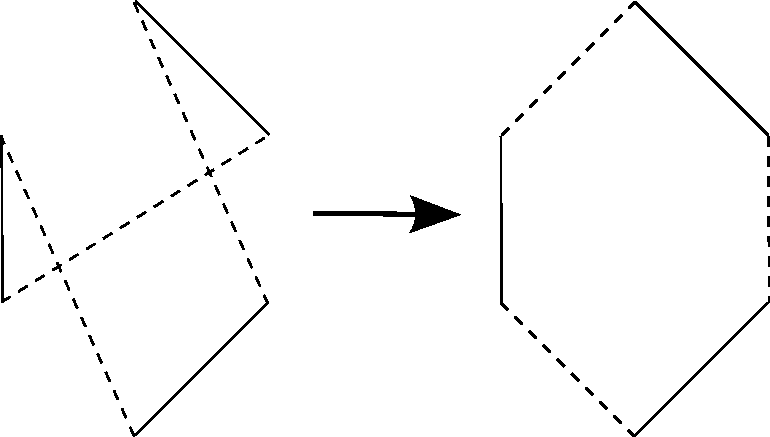
\includegraphics[scale=0.6]{img/opt3.pdf}
\caption{3-opt krok, čiarkovane sú vyznačené hrany, ktoré odstraníme, resp. pridáme}
\end{figure}


Sekvenčné $k$-opt kroky vieme hľadať priamočiaro pomocou rekurzie -- v každom kroku si vyberieme,
ktorú hranu pridáme do množiny $X$ alebo $Y$ (postupujeme striedavo), začíname najprv množinou $X$.
Po pridaní hrany do množiny $X$ skúsime uzavrieť cyklus (ignorujeme, či hrana, ktorá uzavrie
cyklus je z množiny kandidátov). A skontrolujeme, či po takomto ťahu dostaneme stále hamiltonovskú
kružnicu a či jej dĺžka bude kratšia. V momente, keď nájdeme vhodný ťah aplikujeme ho -- t.j.
nehľadáme najlepší $k$-opt ťah.

Zároveň si pri rekurzii počítame doterajší zisk, t.j. rozdiel medzi dĺžkou odobraných a pridaných hrán.
Pokiaľ chceme, aby náš $k$-opt krok bol dobrý, tak jeho zisk musí byť kladný. My použijeme ešte
agresívnejšie orezanie -- požadujeme, aby po každom kroku rekurzie sme malý kladný zisk. Toto vôbec
neobmedzí prehľadané kroky, lebo ak máme celkovo kladný zisk, tak vieme cyklus prejsť v takom
poradí, aby bol zisk po každom kroku kladný.

\medskip

V našom prípade máme hamiltonovské kružnice dve. Priamočiara implementácia by mohla pre každý
$k$-opt ťah kontrolovať, či neporuší podmienku disjuktnosti ciest a povoliť len tie, ktoré ju
neporušujú.

Naše kroky budú mierne komplikovanejšie. Algoritmus na ich nájdenie by sa dal popísať nasledovne:
\begin{enumerate}
\item Nájdi $k$-opt krok v jeden z kružníc, ktorý túto kružnicu zlepší. Nech tento krok vymaže hrany
z množiny $X$ a pridá hrany z množiny $Y$.
\item Ak sa žiadna hrana z množiny $Y$ nenachádza v druhej kružnici, vykonaj tento krok.
\item Ak má prienik druhej kružnice a $Y$ veľkosť 1, tak nájdi v druhej kružnici najlacnejší $2$-opt
alebo $3$-opt krok, ktorý obsahuje túto hranu. Ak sa po vykonaní týchto krokov zlepší súčet dĺžok
kružníc, vykonaj tieto kroky.
\item V prípade, že má tento prienik veľkosť viac ako $1$, označme hrany v prieniku ako $e_1, \dots,
e_k$. Tieto hrany nám druhú kružnicu rozdelia na niekoľko ciest. Vyskúšame všetky možnosti ako tieto
cesty pospájať bez toho, aby sme použili hrany $e_1, \dots, e_k$ a vyberieme najlacnejšiu. Ak sa po
vykonaní týchto krokov zlepší súčet dĺžkov kružníc vykonaj tieto krokov.
\item Ináč nájdi iný $k$-opt krok v prvej kružnici.
\end{enumerate}

Tieto kroky opakujeme kým sa riešenie nedá zlepšiť. Pokiaľ sa zasekneme v lokálnom optime, tak sa pokúsime 
dostať tak, že spravíme niekoľko krokov, ktoré jednu cestu zlepšia a súcet nezhoršia o viac ako
$1\%$. A následne sa opäť snazíme znižovať celkovú dĺžku. Algoritmus skončí vtedy, keď sa už ani
po takýchto krokoch nepodarí riešenie zlepšiť.

\section{Riešenia pomocou celočíselného lineárneho programovania}

Naše riešenie vychádza z riešenia od \cite{duchenne}, ktoré sme stručne opísali v druhej kapitole.
Pripomeňme, že hlavnou myšlienkou tohoto riešenia je hľadať 4-súvislý 4-faktor, ktorý sa následne
pokúšeme rozdeliť na dve hamiltonovské kružnice. Pokiaľ sa toto rozdelenie nepodarí, daný 4-faktor
zakážeme a hľadáme ďalší.

My toto riešenie vylepšíme pomocou niekoľkých vecí.

\subsection{Rozdeľovanie 4-súvislého 4-faktora pomocou SAT solvera}

Ako sme už spomínali zistiť, či sa dá rozdeliť 4-súvislý 4-faktor na dve hamiltonovské kružnice
je NP-úplný problém. Pôvodné riešenie tento problém rieši pomocou celočíselného lineárneho programu.
Keďže ale tento problém je rozhodovací a nie optimalizačný, nám sa zdá rozumnejšie tento 
problém riešiť pomocou SAT solvera. Technika riešenia bude takmer podobná ostatným.
Na začiatku budeme požadovať iba rozklad na dva 2-faktory (t.j. rozložíme hrany do dvoch množín $A,
B$ tak, aby každý vrchol mal dve susedné hrany z $A$ a dve susedné hrany z $B$). Pokiaľ sa vyskytne
nejaký cyklus $C$, ktorý neprechádza celým grafom, tak tento cyklus zakážeme (t.j. budeme požadovať
výskyť aspoň jednej hrany medzi množinami $C$ a $V \setminus C$). 

\subsection{Zrýchlenie rozdeľovania pomocou hľadania vhodných podgrafov}

Už \cite{duchenne} ukázal jeden spôsob ako zrýchliť rozhodovanie, či sa dá 4-súvislý 4-faktor
rozdeliť na dve hamiltonovské kružnice.

\begin{definicia}
Artikulačný pár v 4-súvislom 4-regulárnom grafe $G = (V, E)$ 
je dvojica vrcholov $v_1, v_2$ také, že keď z grafu odstránime
tieto vrcholy a ich susediace hrany, tak sa graf rozpadne na dva grafy
$G_1, G_2$.
\end{definicia}

Artikulačné páry vieme triviálne hľadať v čase $O(n^3)$.

Pokiaľ nájdeme v grafe $G$ artikulačný pár $v_1, v_2$ môžeme ho rozdeliť pomocou nasledovnej
dekompozície:
Nech sa po odstránení vrcholov $v_1, v_2$ graf rozpadne na dva grafy $G_1, G_2$.
Graf $G_1^{'}$ vytvoríme z $G_1$ tak, že mu pridáme vrcholy $v_1, v_2$ a všetky hrany, ktoré spajáli
vrcholy $v_1, v_2$ s grafom $G_1$ v grafe $G$. Následne ešte spojíme vrcholy $v_1, v_2$ medzi sebou
pomocou dvoch hrán. Obdobne vyrobíme z grafu $G_2$ graf $G_2^{'}$.

\begin{figure}
\centering
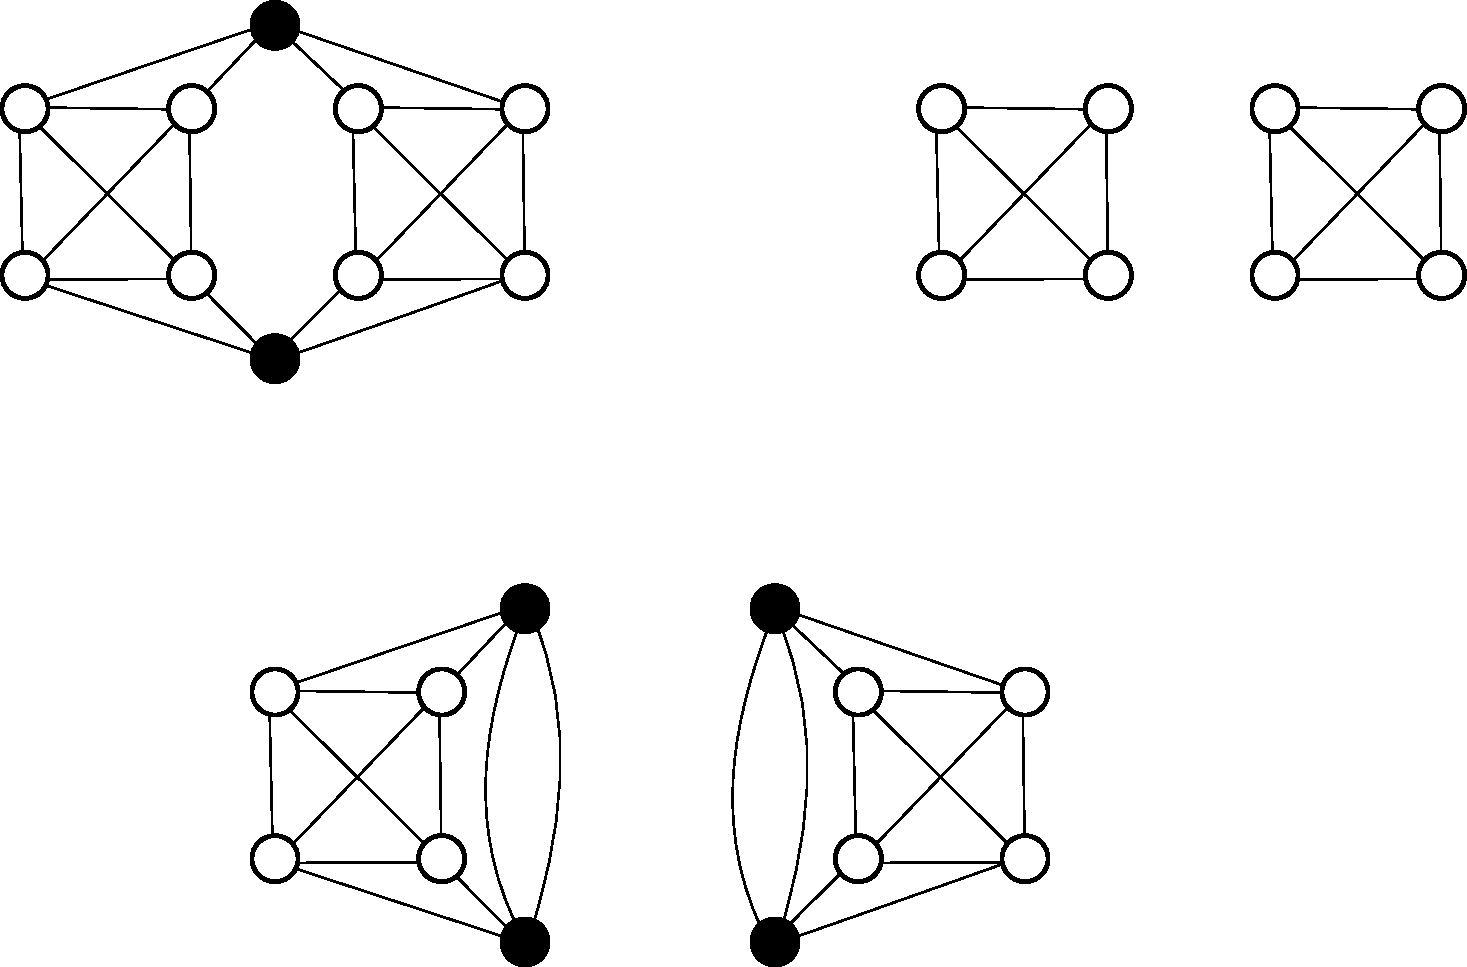
\includegraphics[width=15cm]{img/decomp.pdf}
\caption{Dekompozícia grafu. Hore vľavo: vstupný graf $G$ s vyznačeným artikulačným párom. Hore
vpravo: Graf po odstranení artikulačného páru. Dole: Vzniknuté grafy, po pridaní artikulačným párov
a hrán medzi nimi.}
\end{figure}

Grafy $G_1^{'}, G_2^{'}$ budú 4-súvislé a 4-regulárne. Navyše o nich platí nasledovné.

\begin{veta}
Nech $G$ je 4-súvislý 4-regulárny graf, ktorý obsahuje artikulačný pár $v_1, v_2$.
Nech $G_1^{'}, G_1^{'}$ sú grafy, ktoré vznikli dekompozíciou popísanou vyššie.
Graf $G$ sa dá rozložiť na dve hamiltonovské kružnice práve vtedy a len vtedy, keď
sa grafy $G_1^{'}$ a $G_2^{'}$ dajú rozložiť na dve hamiltonovské kružnice.
\end{veta}

\begin{dokaz}
Pozri \cite{duchenne}.
\end{dokaz}

Túto techniku môžeme aplikovať rekurzívne. Navyše pokiaľ sme spravili iba jednu dekompozíciu, tak
môžeme zakázať menšiu časť grafu ako celý. T.j. ak sa nepodarí daný graf $G$ rozložiť na dve
hamiltonovské kružnice, preto, lebo graf $G_1^{'}$ sa nepodarilo rozložiť, tak môžeme miesto podmienky:
$$\sum_{e \in G} x_e \leq 2n - 1$$

Použiť podmienku:
$$\sum_{e \in G_1^{'}} x_e \leq |E_1^{'}| - 1$$

Táto technika ale nefunguje rekurzívne, ale iba pri prvej dekompozícii.

\medskip

V našom algoritme používame ešte jednu operáciu, ktorá vstup pre SAT solver ešte zjednoduší.
Myšlienka vyzerá nasledovne: Ak nájdeme nejakú štvorcu bodov, ktoré sú všetky navzájom spojené
(kliku veľkosti 4), tak
ich môžeme zlučiť do jedného bodu.

\begin{veta}
Nech $G$ je 4-súvislý 4-regulárny graf a nech $v_1, v_2, v_3, v_4$ sú jeho vrcholy také, že medzi
každými dvoma vedie hrana. Nech graf $G^{'}$ vznikne z grafu $G$ tak, že vrcholy $v_1, v_2, v_3,
v_4$ zlúčime do jedného. Potom graf $G$ je rozložiteľný na dve hamiltonovské kružnice práve vtedy a
len vtedy, keď je graf $G^{'}$ rozložiteľný na dve hamiltonovské kružnice.
\end{veta}

\begin{dokaz}
Zoberme hrany, ktoré vedú medzi množinami $V_x = \{v_1, v_2, v_3, v_4\}$ a $V \setminus V_x$.
Takéto hrany sú práve 4. Ak by ich bolo menej, tak $G$ nie je 4-súvislý, ak by ich bolo viac, tak
$G$ nemôže byť 4-regulárny.

Ak sa graf $G$ dá rozložiť na dve hamiltonovské kružnice, tak triviálne vidno, že aj graf $G^{'}$ sa
dá rozložiť (kružnice budú presne rovnaké akuráť vynecháme hrany medzi vrcholmi $v_1, \dots, v_4$).

\begin{figure}[h]
\centering
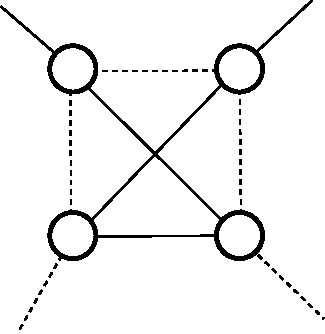
\includegraphics[scale=0.5]{img/k4.pdf}
\caption{Prechod kružníc cez kliku veľkosti 4}
\label{fig:k4}
\end{figure}

Ak sa graf $G^{'}$ dá rozložiť na dve hamiltonovské kružnice, tak pomocou vhodného prepojenia (viď.
\ref{fig:k4}) medzi
vrcholmi $v_1, \dots, v_4$ vieme graf $G$ rozložiť na dve hamiltonovské kružnice (ostatné hrany
rozložíme medzi kružnice rovnako ako v grafe $G^{'}$).
\end{dokaz}

Poznamenajme, že takéto štvorice vrcholov vieme hľadať v čase $O(n)$ -- vyberieme si jeden vrchol
$v_1$ a v konštantom čase prejdeme všetky jeho kombinácie susedov.

\subsection{Odstráňovanie nepoužiteľných hran}

Predstavme si graf, ktorého vrcholy zodpovedajú bodom v rovine. Pomerne intuitívne vieme označiť
veľa hrán, o ktorých si sme istý, že v optimálnom riešení určite nebudú -- sú to hlavne tie hrany,
ktoré vedú cez celú rovinu. My by sme v tejto časti chceli ukázať ako tieto hrany
hľadať algoritmicky. Pokiaľ by sme ich vedeli hľadať, môžeme obmedziť počet premenných, ktoré
sú v lineárnom programe a tak urýchliť jeho riešenie.

\begin{lema}
Nech $l(G, e)$ je dolný odhad veľkosti riešenia, ktoré obsahuje hranu $e$.
Nech $u(G)$ je nejaký horný odhad riešenia. Ak $l(G, e) > u(G)$, tak sa hrana $e$ určite nepoužije v
optimálnom riešení.
\end{lema}

\begin{dokaz}
Triviálny.
\end{dokaz}

Ako získať horný odhad veľkosti riešenia sme už popísali. Ešte potrebujeme popísať ako získať dolný
odhad, ktorý obsahuje hranu $e$.

\medskip
Pokiaľ používame dolný odhad pomocou štyroch najbližších susedov, tak sa dolný odhad, ktorý obsahuje
hranu $e$ dá získať pomerne jednoducho. Nech $e$ vedie medzi vrcholmi $x, y$. Potom do veľkosti
dolného odhadu miesto $4$ najbližších susedov započítame iba $3$ najbližších susedov (okrem hrany
$e$) a navyše hranu $e$ započítame $2-krát$. Pokiaľ máme už dopredu spočítaný dolný odhad bez nutnej
hrany, tak pre danú hranu $e$ vieme tento odhad prerátať v konštantnom čase. 
To znamená, že v čase $O(n^2)$ vieme nájsť nepoužiteľné hrany. 

\medskip
Pokiaľ používame dolný odhad pomocou dvoch disjuktných kostier, tak je situácia trochu zložitejšia.
Pokiaľ máme spočítané najlacnejšie dve disjuktné kostry a chceme, aby sa nutne použila hrana $e$,
tak potrebujeme z týchto kostier jednu hranu vyhodiť. Nestačí sa ale len pozrieť na cykly v ktorých
leží hrana $e$, lebo môžeme si hrany medzi kostrami presúvať. To znamená, že vložime hranu $e$, inú
hranu $e_1$ presunieme z kostry $M_1$ do kostry $M_2$ ($e$ a $e_1$ ležali po pridaní do $M_1$ na
jednom cykle), ďalšiu hranu $e_2$ presunieme z $M_2$ do $M_1$, atď., až nakoniec odstraníme hranu
$e_k$. Teda hľadáme cestu medzi hranami kostier a chceme vyhodiť najlacnejšiu hranu, ku ktorej sa
vieme dostať. Tento problém efektívne rieši značkovacia procedúra z \cite{spanning2}, akurát si
potrebujeme pamätať akú najlacnejšiu hranu vieme dosiahnúť. Táto značkovacia procedúra trvá pre
jednu hranu čas $O(n)$. Následne keď zistíme, ktorú hranu musíme z kostier vyhodiť, tak
veľkosti dolného odhadu vieme prerátať triválne. Celkovo na to, aby sme o každej hrane zistili či
je zbytočná potrebujeme čas $O(n^3)$. 

\begin{poznamka}
Dobre spravený algoritmus by toto vedel riešiť aj v čase $O(n^2)$. Keďže ale vo všetkých
naších vstupoch platí $n \leq 500$, tak je $O(n^3)$ riešenie postačujúce a nepotrebujeme sa zaoberať
komplikovanejším riešením.
\end{poznamka}

\section{Experimenty}

Vyššie popísané algoritmy sme implementovali s cieľom empiricky overiť ich účinnosť na
niektorých druhoch dát. Testovacie dáta budú tvoriť náhodné grafy v euklidovskej rovine (kde
súradnice bodov sú vyberané rovnomerne náhodne) a niektoré inštancie z TSPLIB (\cite{tsplib}).

Hľadanie dolných a horných odhadov sme implementovali v C++. Na riešenie celočíselných
lineárnych programov sme použili Numberjack, ktorý používa SCIP a ako SAT solver sme použili knižnicu STP, ktorá
používa MINISAT. Réžiu okolo celočíselných lineárnych programov a SAT solvera sme
implementovali v jazyku Python. 

Testovali sme tri rôzne implementácie. Jedna nepoužívala žiadne vyhadzovanie nepotrebných
hrán, druhá používala vyhadzovanie nepotrebných hrán cez štyroch najbližších susedov a tretia
používala vyhadzovanie nepotrebných hrán pomocou dvoch disjuktných kostier.

V prípade náhodných grafov v euklidovskej rovine sme generovali grafy veľkosti $100$, $150$, $200$,
$250$, $300$. Pre každú veľkosť sme vygenerovali 10 grafov.
Následne sme každú našu implementáciu pustili a sledovali niekoľko údajov:
\begin{itemize}
\item Či úspešne skončí do jednej hodiny. Ak neskončí, tak rátame riešenie za neúspešné.
\item Ako rýchlo skončí.
\item Koľko krát sa vykoná rozklad 4-súvislého 4-faktora na dve hamiltonovské kružnice.
\item Koľko hrán bolo označených ako nepoužiteľné.
\end{itemize}

V prípade, že sme používali odhady, sme navyše počítali aj relatívne rozdiely
medzi dolným a horným odhadom, resp. medzi odhadmi a optimálnym riešením.

\subsection{Výsledky pre náhodny grafy v euklidovskej rovine}

V tabuľke \ref{TODO} sú zhrnuté priemerné výsledky pre každú veľkosť grafu.
Označenia: 
\begin{myitemize}
\item $n$ -- veľkosť grafu
\item $f_a$ -- priermerný počet rozkladov na dve hamiltonovské kružnice pre všetky
inštancie (v prípade, že sme do hodiny nedostali výsledok, tak rátame počet rozkladov, ktoré program
stihol vykonať za hodinu)
\item $f_u$ -- priemerný počet rozkladov pre inštancie, kde sme úspešne skončili
\item $f_1$ -- počet inštancií, kde prvý rozklad bol úspešný 
\item $s_n$ -- uspešnosť algoritmu, keď sme žiadne nepotrebné hrany nehľadali
\item $t_n$ -- priemerný čas behu algoritmu, keď sme žiadne nepotrebné hrany nehľadali (pokiaľ sme
neskončili v priebehu hodiny, do priemeru zarátame hodinu) v sekundách
\item $u_n$ - to isté, čo $t_u$ ale rátame priemer iba na inštanciách, kde sme úspešne skončili
\item $s_4, t_4, u_4$ -- úspešnosť a časy behu v prípade, že nepoužiteľné hrany, hľadáme pomocou
štyroch najbližších susedov
\item $d_4$ -- priemerný podiel nájdených nepoužíteľných hrán
\item $s_k, t_k, u_k$ -- úspešnosť a časy behu v prípade, že nepoužiteľné hrany, hľadáme pomocou
dvoch disjuktných kostier
\item $d_k$ -- priemerný podiel nájdených nepoužíteľných hrán
\end{myitemize}



\begin{table}[h]
\centering
\begin{tabular}{|r|r|r|r|r|r|r|r|r|r|r|r|r|r|r|}
\hline
$n$&$f_a$&$f_u$&$f_1$&$s_n$&$t_n$&$u_n$&$s_4$&$t_4$&$u_4$&$d_4$&$s_k$&$t_k$&$u_k$&$d_k$ \\\hline
100& 57  & 29  & 5   & 0.9 & 736 & 378 & 0.9 & 687 & 322 & 0.64& 0.9 & 585 & 249 & 0.63 \\\hline
150& 83  & 28  & 4   & 0.7 & 1380& 428 & 0.7 & 1327& 353 & 0.61& 0.7 & 1318& 334 & 0.53 \\\hline
200& 68  & 8   & 3   & 0.5 & 2000& 400 & 0.5 & 1903& 206 & 0.56& 0.5 & 1924& 226 & 0.51 \\\hline
250& 46  & 22  & 2   & 0.3 & 2769& 819 & 0.4 & 2662& 1255& 0.50& 0.4 & 2630& 1136& 0.45 \\\hline
\end{tabular}
\caption{Výsledky pre náhodné grafy.}
\end{table}


%\chapter{Rozhranie knižnice}
%\label{chapter:rozhranie}
%\input{tex/10reference.tex}
%\input{tex/11containers.tex}
%\input{tex/12ordered_containers.tex}
%\input{tex/13unordered_containers.tex}
%\input{tex/14array_utils.tex}
%
%\chapter{Implementácia}
%\label{chapter:implementation}
%\input{tex/21sequence_implementation.tex}
%\input{tex/22ordered_implementation.tex}
%\input{tex/23unordered_implementation.tex}
%\input{tex/24sorting.tex}
%\input{tex/25testing.tex}
%
%\chapter{Praktické testy}
%\label{chapter:practical}
%\input{tex/3practical.tex}
%\input{tex/31sorting.tex}
%\input{tex/32lcs.tex}
%\input{tex/33asfalt.tex}
%\input{tex/34basnik.tex}
%\input{tex/35conclusion.tex}

\chapter*{Záver}
\addcontentsline{toc}{chapter}{Záver}
\label{chapter:fin}
V tejto práci sme zhrnuli a navrhli niekoľko nových prístupov
pre riešenie problému dvoch obchodných cestujúcich.
Naše hlavné prínosy sú nasledovné:
\begin{itemize}
\item Navrhli sme exaktný algoritmus, ktorého časová zložitosť je oveľa
lepšia ako zložitosť triviálneho algoritmu.
\item Ukázali sme ako urobiť PTAS pre problém dvoch obchodných cestújich.
Navyše jeho zložitosť nie je horšia ako zložitosť PTASu pre problém obchodného
cestujúceho.
\item Navrhli sme niekoľko heuristík a porovnali ich s doterajšími.
Kým doterajšie heuristiky zvládali inštancie s maximálnou veľkosťou 280, naše
heuristiky zvládajú inštancie s maximálnou veľkosťou 442.
\end{itemize}

V spomínaných výsledkoch je stále niekoľko miest na zlepšenie.
Pri exaktnom algoritme je zaujímavé zistiť, či obmedzenie na vstupný graf
(napr. trojuholníková nerovnosť) neumožní návrh ešte rýchlejšieho algoritmu.
Pri heuristikách by bolo veľmi nápomocné, ak by sa podarilo nájsť postup
ako znížiť počet zistovaní toho, či je 4-súvislý 4-regulárny graf rozložiteľný
na dve hamiltonovské kružnice.


%\chapter{Prehľad štandardných algoritmov - obsolete, nema tu co robit} 
%\label{chapter:salg}
%\input{tex/x1sorting.tex}
%\input{tex/x2containers.tex}
%\input{tex/x3sets.tex}

%\backmatter fixme: preco to tu nefunguje? asi chyba nejaky package
%\listoffigures
%\listoftables

\bibliographystyle{alpha}
\bibliography{literatura}



\end{document}
